%%=============================================================================
%% LaTeX sjabloon voor bachelorproef, HoGent Bedrijf en Organisatie
%% Opleiding Toegepaste Informatica
%%=============================================================================

\documentclass[pdftex,a4paper,12pt,twoside]{report}

%% TODO: Let op: dit sjabloon is ontworpen om dubbelzijdig af te drukken, met
%% asymmetrische marges. Voor enkelzijdig, verwijder ``twoside'' hierboven.

%%=============================================================================
%% LaTeX sjabloon voor de bachelorproef, HoGent Bedrijf en Organisatie
%% Opleiding toegepaste informatica
%%
%% Structuur en algemene vormgeving. Meestal hoef je hier niets te wijzigen.
%%
%% Auteur: Bert Van Vreckem <bert.vanvreckem@hogent.be>
%% Licentie: CC-BY https://creativecommons.org/licenses/by/4.0/
%%=============================================================================

%%---------- Packages ---------------------------------------------------------

\usepackage[utf8]{inputenc}  % Accenten gebruiken in tekst (vb. é ipv \'e)
\usepackage{amsfonts}        % AMS math packages: extra wiskundige
\usepackage{amsmath}         %   symbolen (o.a. getallen-
\usepackage{amssymb}         %   verzamelingen N, R, Z, Q, etc.)
\usepackage[english,dutch]{babel}    % Taalinstellingen: woordsplitsingen,
                             %  commando's voor speciale karakters
                             %  ("dutch" voor NL)
\usepackage{iflang}
\usepackage{eurosym}         % Euro-symbool €
\usepackage{geometry}
\usepackage{graphicx}        % Invoegen van tekeningen
\usepackage[pdftex,bookmarks=true]{hyperref}
                             % PDF krijgt klikbare links & verwijzingen,
                             %  inhoudstafel

\usepackage{listings}        % Broncode mooi opmaken
\usepackage[T1]{fontenc}
\usepackage[scaled]{beramono}

\usepackage{color}
\definecolor{bluekeywords}{rgb}{0.13,0.13,1}
\definecolor{greencomments}{rgb}{0,0.5,0}
\definecolor{redstrings}{rgb}{0.9,0,0}

\usepackage{listings}
\lstset{language=[Sharp]C,
showspaces=false,
showtabs=false,
breaklines=true,
showstringspaces=false,
breakatwhitespace=true,
escapeinside={(*@}{@*)},
commentstyle=\color{greencomments},
keywordstyle=\color{bluekeywords}\bfseries,
stringstyle=\color{redstrings},
basicstyle=\ttfamily
}
\usepackage{multirow}        % Tekst over verschillende cellen in tabellen
\usepackage{rotating}        % Tabellen en figuren roteren
\usepackage{natbib}          % Betere bibliografiestijlen
\usepackage{fancyhdr}        % Pagina-opmaak met hoofd- en voettekst

\usepackage[T1]{fontenc}     % Ivm lettertypes
\usepackage{lmodern}
\usepackage{textcomp}

\usepackage{etoolbox}
\usepackage{lipsum}          % Voor vultekst (lorem ipsum)

%%---------- Layout -----------------------------------------------------------

\pagestyle{fancy}                % Hoofdingen invoegen
\renewcommand{\sectionmark}[1]{} % Enkel hoofdstuktitel in hoofding, geen
                                 % sectietitel (vermijd overlap)

% Leeg blad
\newcommand{\emptypage}{
\newpage
\thispagestyle{empty}
\mbox{}
\newpage
}

% Gebruik een schreefloos lettertype ipv het "oubollig" uitziende
% Computer Modern
\renewcommand{\familydefault}{\sfdefault}

%%---------- Broncode (Java) --------------------------------------------------
% Commando voor invoegen Java-broncodebestanden (dank aan Niels Corneille)
% Gebruik:
%   \codefragment{source/MijnKlasse.java}{Uitleg bij de code}
%
% Je kan dit aanpassen aan de taal die je zelf het meeste gebruikt in je
% bachelorproef.
\newcommand{\codefragment}[2]{ \lstset{%
  language=java,
  breaklines=true,
  float=th,
  caption={#2},
  basicstyle=\scriptsize,
  frame=single,
  extendedchars=\true
}
\lstinputlisting{#1}}


%%---------- Voorblad ---------------------------------------------------------

\newcommand{\inserttitlepage}{%
\begin{titlepage}
  \newgeometry{top=2cm,bottom=1.5cm,left=1.5cm,right=1.5cm}
  \begin{center}

    \begingroup
    \rmfamily
    
\includegraphics[width=2.5cm]{img/HG-beeldmerk-woordmerk}\\[.5cm]
    Faculteit Bedrijf en Organisatie\\[3cm]
    \titel
    \vfill
    \student\\[3.5cm]
    Scriptie voorgedragen tot het bekomen van de graad van\\professionele bachelor in de toegepaste informatica\\[2cm]
    Promotor:\\
    \promotor\\
    \ifdefempty{\copromotor}{\vspace{2.5cm}}{Co-promotor:\\\copromotor\\[2.5cm]}
    Instelling: \instelling\\[.5cm]
    Academiejaar: \academiejaar\\[.5cm]
    \ifcase \examenperiode \or Eerste \or Tweede \else Derde \fi examenperiode
    \endgroup

  \end{center}
  \restoregeometry
\end{titlepage}
  \emptypage
\begin{titlepage}
  \newgeometry{top=5.35cm,bottom=1.5cm,left=1.5cm,right=1.5cm}
  \begin{center}

    \begingroup
    \rmfamily
    \IfLanguageName{dutch}{Faculteit Bedrijf en Organisatie}{Faculty of Business and Information Management}\\[3cm]
    \titel
    \vfill
    \student\\[3.5cm]
    \IfLanguageName{dutch}{Scriptie voorgedragen tot het bekomen van de graad van\\professionele bachelor in de toegepaste informatica}{Thesis submitted in partial fulfillment of the requirements for the degree of\\professional bachelor of applied computer science}\\[2cm]
    Promotor:\\
    \promotor\\
    \ifdefempty{\copromotor}{\vspace{2.5cm}}{Co-promotor:\\\copromotor\\[2.5cm]}
    \IfLanguageName{dutch}{Instelling}{Institution}: \instelling\\[.5cm]
    \IfLanguageName{dutch}{Academiejaar}{Academic year}: \academiejaar\\[.5cm]
    \IfLanguageName{dutch}{%
    \ifcase \examenperiode \or Eerste \or Tweede \else Derde \fi examenperiode}{%
    \ifcase \examenperiode \or First \or Second \else Third \fi examination period}
    \endgroup

  \end{center}
  \restoregeometry
\end{titlepage}
}


%%---------- Documenteigenschappen --------------------------------------------
%% TODO: Vul dit aan met je eigen info:

%% Je eigen naam
\newcommand{\student}{Yannick Van Hecke}

%% De naam van je promotor (lector van de opleiding)
\newcommand{\promotor}{Koen Hoof}

%% De naam van je co-promotor. Als je promotor ook je opdrachtgever is en je dus ook inhoudelijk begeleidt, mag je dit leeg laten.
\newcommand{\copromotor}{Jeroen Gevenois}

%% Indien je bachelorproef in opdracht van/in samenwerking met een bedrijf of
%% externe organisatie geschreven is, geef je hier de naam. Zoniet laat je dit
%% zoals het is.
\newcommand{\instelling}{Politiezone Gent - Dienst ICT}

% De titel van het rapport/bachelorproef
\newcommand{\titel}{Vergelijkende studie en proof-of-concept in functie van een doelbewuste keuze tussen een cross platform mobiele applicatie en een mobiele website}

% Datum van indienen (gebruik telkens de deadline, ook al geef je eerder af)
\newcommand{\datum}{2 juni 2017}

% Academiejaar
\newcommand{\academiejaar}{2016-2017}

% Examenperiode
%  - 1e semester = 1e examenperiode => 1
%  - 2e semester = 2e examenperiode => 2
%  - tweede zit  = 3e examenperiode => 3
\newcommand{\examenperiode}{2}

%%=============================================================================
%% Inhoud document
%%=============================================================================

\begin{document}

%% Als je je bachelorproef in het Engels schrijft, haal dan onderstaande regel
%% uit commentaar. Let op: de tekst op de voorkaft blijft in het Nederlands, en
%% dat is ook de bedoeling!
%\selectlanguage{english}

\inserttitlepage
%% hallo
%%=============================================================================
%% Samenvatting
%%=============================================================================

%% TODO: De "abstract" of samenvatting is een kernachtige (~ 1 blz. voor een
%% thesis) synthese van het document.
%%
%% Deze aspecten moeten zeker aan bod komen:
%% - Context: waarom is dit werk belangrijk?
%% - Nood: waarom moest dit onderzocht worden?
%% - Taak: wat heb je precies gedaan?
%% - Object: wat staat in dit document geschreven?
%% - Resultaat: wat was het resultaat?
%% - Conclusie: wat is/zijn de belangrijkste conclusie(s)?
%% - Perspectief: blijven er nog vragen open die in de toekomst nog kunnen
%%    onderzocht worden? Wat is een mogelijk vervolg voor jouw onderzoek?
%%
%% LET OP! Een samenvatting is GEEN voorwoord!

%%---------- Nederlandse samenvatting -----------------------------------------
%%
%% TODO: Als je je bachelorproef in het Engels schrijft, moet je eerst een
%% Nederlandse samenvatting invoegen. Haal daarvoor onderstaande code uit
%% commentaar.
%% Wie zijn bachelorproef in het Nederlands schrijft, kan dit negeren en heel
%% deze sectie verwijderen.


%%---------- Samenvatting -----------------------------------------------------
%%
%% De samenvatting in de hoofdtaal van het document

\begin{abstract}
  %%\lipsum[1-4]

  Deze bachelorproef heeft als doel de ontwikkelaar op basis van onderzoek naar ontwikkeltijd, kosten, snelheid en gegevensverbruik
  te helpen in de keuze tussen een cross platforme mobiele applicatie en responsive website. Dit omdat er vandaag de dag weinig artikels
  ter beschikking zijn waarin een gefundeerde keuze wordt gemaakt voor 1 van beide vormen van toepassingen.

  Dit werk is tot stand gekomen in verschillende fases. Zo werd er eerst een literatuuronderzoek verricht naar eerdere vergelijkende
  studie tussen cross platforme mobiele apps en responsive websites.

  Na het vastleggen van de casus werd er gekozen voor Visual Studio als ontwikkelingomgeving, waarna de ontwikkeling van beide toepassingen volgde. Eens de ontwikkeling afgerond was, werden de tijden voor
  opstarten, inloggen en gegevens ophalen gemeten samen met de hoeveelheid gegevens die dit met zich meebrengt. Dit om nadien een
  gefundeerde conclusie te vormen op basis van snelheid, gegevensverbruik, kosten. Dit alles zonder caching van data in de mobiele applicatie.

  Uit de resultaten van het onderzoek kwam naar voor dat indien men het gegevensverbruik van de toepassing een belangrijk kenmerk vindt, men
  beter kiest voor de mobiele applicatie. Voor de snelheid van de toepassing, heeft bij Android
  de responsive website een duidelijk voordeel ten opzicht van de mobiele applicatie. Bij windowsphone was mobiele applicatie sneller.
  In het iOS-project is wegens tijdgebrek enkel het inloggen gedeeltelijk geïmplementeerd. Hierop werden geen testen uitgevoerd.

  Verder worden ook de kosten om beide toepassingen te hosten in rekening genomen. voor de mobiele applicatie komt dit voor de web api € 92,56 per maand.
  Hierbij moeten nog de kosten voor publicatie in de applicatiewinkel meegerekend worden. Voor android is dit eenmalig 25 dollar. Voor windowsphone is
  dit € 16,98 (19 dollar) voor een individueel account en € 88,50 (99 dollar) voor een bedrijfsaccount. De kost voor de iOS-applicatie te publiceren komt op 99 dollar per jaar.
  Indien deze kosten van belang zijn, kiest men beter voor de responsive webapplicatie. Dit omdat hier enkel de € 92,56 per maand erbij komt.
  Dit naast de kosten voor een macOS-toestel om de iOS-applicatie op te testen.

  De snelheid van ontwikkeling is een criterium dat ook in rekening werd gebracht in deze vergelijkende studie.
  Hierbij was het resultaat dat bij de responsive website sneller tot een gebruiksklaar eindproduct kon komen.
  Dit terwijl men bij de mobiele applicatie drie afzonderlijke deelprojecten moest maken. De uitgebereide resultaten en conclusies
  worden meer in detail toegelicht in de scriptie.



\end{abstract}

%%=============================================================================
%% Voorwoord
%%=============================================================================

\chapter*{Voorwoord}
\label{ch:voorwoord}

%% TODO:
%% Het voorwoord is het enige deel van de bachelorproef waar je vanuit je
%% eigen standpunt (``ik-vorm'') mag schrijven. Je kan hier bv. motiveren
%% waarom jij het onderwerp wil bespreken.
%% Vergeet ook niet te bedanken wie je geholpen/gesteund/... heeft

In deze bachelorproef worden de verschillen in performantie tussen een cross-platforme mobiele applicatie en responsive website onderzocht.
De keuze voor dit onderwerp is gekomen na een opdrachtswijziging in de stage van het vorige academiejaar (2015-2016).

Toen werd er na een kostenanalyse van een cross-platforme mobiele applicatie beslist om over te schakelen op een responsive website.
Het was dan dat mijn interesse om dit uitgebereider te onderzoeken, getriggerd werd.

Deze vergelijkende studie en proof-of-concept in functie van een doelbewuste keuze tussen een cross platforme mobiele applicatie en
een mobiele website werd gevoerd tussen februari 2017 en mei 2017 bij de ICT-afdeling van de Gentse Politie.

Daarom wens ik ook mijn dank te betuigen aan mijn co-promotor Jeroen Gevenois om mij steeds bij te staan tijden mijn onderzoeken en voor
het beantwoorden van mijn vragen tijdens het ontwikkelen van beide toepassingen.
op mijn vragen tijdens het ontwikkelen van beide toepassingen.

Ook wil ik ook Matthias Vercaemst bedanken om mij te helpen met de verschillende netwerken-vragen die ik had tijdens het onderzoek.

Ook diensthoofd Ruben Vansevenant zou ik graag willen vermelden in mijn bedankingen omdat hij mij de kans te geven om deze bachelorproef uit te werken.

Verder wil ik ook mijn promotor Koen Hoof bedanken voor de steeds opbouwende feedback en de stipte opvolging van deze bachelorproef tijdens de afgelopen maanden.
Deze feedback hielp mij om telkens weer dit werk te verbeteren.

Tot slot bedank ik nog mijn Gon-Begeleider Elke Van Paemel voor de steun tijdens het schrijven van de bachelorproef.


\tableofcontents

%% Als je een lijst van afkortingen of termen wil toevoegen, dan hoort die
%% hier thuis. Gebruik bijvoorbeeld de ``glossaries'' package.

%%---------- Kern -------------------------------------------------------------


%%=============================================================================
%% Inleiding
%%=============================================================================

\chapter{Inleiding}
\label{ch:inleiding}

%% De inleiding moet de lezer alle nodige informatie verschaffen om het onderwerp te begrijpen zonder nog externe werken te moeten raadplegen \citep{Pollefliet2011}. Dit is een doorlopende tekst die gebaseerd is op al wat je over het onderwerp gelezen hebt (literatuuronderzoek).

%% Je verwijst bij elke bewering die je doet, vakterm die je introduceert, enz. naar je bronnen.
%% In \LaTeX{} kan dat met het commando \texttt{$\backslash${cite\{\}}} of \texttt{$\backslash${citep\{\}}}.
%%Als argument van het commando geef je de ``sleutel'' van een ``record'' in een bibliografische databank in het Bib\TeX{}-formaat
%% (een tekstbestand). Als je expliciet naar de auteur verwijst in de zin, gebruik je \texttt{$\backslash${}cite\{\}}.
%% Soms wil je de auteur niet expliciet vernoemen, dan gebruik je \texttt{$\backslash${}citep\{\}}.
%%Hieronder een voorbeeld van elk.

\section{Stand van zaken}
\label{sec:stand-van-zaken}

%% TODO: deze sectie (die je kan opsplitsen in verschillende secties) bevat je
%% literatuurstudie. Vergeet niet telkens je bronnen te vermelden!
In de vakliteratuur zijn er vandaag diverse artikelen te vinden over een vergelijkende studie tussen mobiele applicatie
en responsive webapplicaties. Meeste onderzoeken die tot nu toe gevoerd zijn, zijn echter een beperkte lijst van kenmerken die aangeven wanneer men het best voor welke optie kiest.
Dit zonder dat hier wetenschappelijk onderzoek aan vooraf ging.

Toch zijn deze wetenschappelijke artikelen beschikbaar. Zo onderzocht \cite{albuquerque2015}
in het artikel 'CROSS PLATFORM APP A COMPARATIVE STUDY' de voornaamste reden om te kiezen voor enerzijds de mobiele
applicatie en anderzijds de responsive website.

De belangrijkste redenen uit het onderzoek om te kiezen voor een cross-platform mobiele applicatie zijn de volgende:
\begin{itemize}
  \item{Performantie}
  \item{User Interfaces in de lijn van het besturingssysteem}
  \item{Distributie via de app stores}
  \item{Push notificaties}
\end{itemize}

In de vakliteratuur haalt men voor de hoofdzakelijkste redenen om te kiezen voor een responsive webapplicatie, de volgende aan:
\begin{itemize}
  \item{Eenvoudige ondersteuning voor meerdere systemen}
  \item{Het publiceren van de toepassing}
\end{itemize}



\section{Probleemstelling en Onderzoeksvragen}
\label{sec:onderzoeksvragen}

%% TODO:
%% Uit je probleemstelling moet duidelijk zijn dat je onderzoek een meerwaarde
%% heeft voor een concrete doelgroep (bv. een bedrijf).
%%
%% Wees zo concreet mogelijk bij het formuleren van je
%% onderzoeksvra(a)g(en). Een onderzoeksvraag is trouwens iets waar nog
%% niemand op dit moment een antwoord heeft (voor zover je kan nagaan).

Momenteel worden er bij de ICT-afdeling van de Gentse Politie aan verschillende projecten gewerkt waarbij het
mobiel beschikbaar maken van interne gegevens een vereiste is.
Om dit naar een gebruiksklaar eindproduct voor een mobiel apparaat om te zetten, bestaan er vandaag de twee opties.

Enerzijds kan er gekozen worden voor een cross-platform mobiele applicatie.
Dit houdt in dat men binnen 1 ontwikkelomgeving een applicatie ontwikkelt die bruikbaar is op de
3 grote mobiele platformen: Android van Google, iOS van Apple en windowsphone of
Windows Universal Platform van Microsoft.
Hierbij wordt er code gedeeld tussen de 3 platformen.

Het weergeven van de data gebeurd op een platform-specifieke manier.
Dit omdat men binnen de verschillende mobiele besturingssystemen werkt met andere UI elementen om de data in te tonen.

Anderzijds bestaat de mogelijkheid om te kiezen voor een responsive webapplicatie.
Dit wil zeggen dat de inhoud van de webapplicatie aangepast wordt,
 naargelang het scherm waarbij men de mobiele website bekijkt.
Zo wordt er op een smartphone mogelijks minder informatie weergegeven dan indien men de website bekijk op een computer of
wordt in het geval van de smartphone de positie en afmetingen van de elementen aangepast.

In dit werk wordt onderzocht in welke gevallen de webapplicatie de beste optie is alsook in welke gevallen de mobiele applicatie
een beter alternatief vormt.

Hierbij zullen volgende onderzoeksvragen beantwoord worden:
\begin{itemize}
  \item{Bij welke vorm van applicatie wordt het snelst resultaat behaald?}
  \item{Welke optie is het meest gebruiksvriendelijk?}
  \item{Welke optie is het efficiënst?}
  \begin{itemize}
    \item{Welke optie verbruikt de meeste hoeveelheid gegevens?}
    \item{Welke optie geeft de eindgebruiker het snelst de gevraagd informatie?}
  \end{itemize}
  \item{Welke optie is het veiligst?}
  \item{Welke optie kan het snelst ontwikkeld worden?}
\end{itemize}
\newpage
\section{Opzet van deze bachelorproef}
\label{sec:opzet-bachelorproef}

In functie van de snelheid van de ontwikkeling van beide producten, moet er een ontwikkelomgeving gekozen worden.
Om een cross-platform mobiele applicatie te ontwikkelen, bestaat de keuze uit 2 technologieën . Enerzijds zijn er
ontwikkelomgeving met C\# als achterliggende programmeertaal. Hierbij wordt de UI gedefinieërd in xml voor Android,
xaml van windowsphone en Universal Windows Platform en storyboards voor iOS. Hierbij wordt de oorspronkelijke interactie
en structuur van de UI en de logica van het mobiele besturingssysteem behouden. Visual Studio en Xamarin zijn 2 voorbeelden
die gebaseerd zijn op deze technologie. Anderzijds kan men ook opteren voor een cross-platforme mobiele applicatie te bouwen op basis van html, css en javascript.
Hierbij wordt er eerst een webservice van het te hosten project gemaakt, om vervolgens deze webservice op te starten in een emulator.
De ontwikkelomgeving PhoneGap is op deze manier van werken gebaseerd.

In dit onderzoek zal gekozen worden voor de eerste manier van werken, nl. de ontwikkelomgeving met C\# als achterliggende
programmeertaal. Vanwege de huidige kennis van het ontwikkelen van cross-platforme mobiele applicatie geniet de eerste optie de voorkeur.

Nadat de gekozen ontwikkelingomgeving vastligt, wordt er aan de hand van de functionele requirements beslist welke de
minimale versies van de besturingssystemen zijn. Hierbij wordt getracht het aantal ondersteunende apparaten zo hoog mogelijk te houden.
Tijdens het onderzoek wordt, zoals in de onderzoeksvragen reeds vermeld, ook rekening gehouden met de tijd en kosten die de ontwikkeling
en publiek stellen van beide applicaties met zich meebrengen.

Vervolgens wordt de gebruikte methodologie verklaard, waarna de casus uitgelegd wordt.
Deze casus is de basis die zal gebruikt wordt in het onderzoek naar efficiëntie en gebruiksvriendelijkheid van de
cross-platforme mobiele applicatie en de responsive webapplicatie.

Nadat de casus duidelijk verklaard is, worden de gemaakte applicaties verklaard aan de hand van de geschreven code.
Vervolgens worden de resultaten getoond en wordt de conclusie die uit het onderzoek voortvloeit, medegedeeld.
Deze conclusie wordt ook gebruikt door de Gentse Politie in hun keuze tussen een mobiele applicatie of een responsive website.

Na de conclusie worden er nog richtlijnen voor toekomstig onderzoek gegeven in deze materie.

%% TODO: Het is gebruikelijk aan het einde van de inleiding een overzicht te
%% geven van de opbouw van de rest van de tekst. Deze sectie bevat al een aanzet
%% die je kan aanvullen/aanpassen in functie van je eigen tekst.
 %% 1
%%=============================================================================
%% Methodologie
%%=============================================================================

\chapter{Methodologie}
\label{ch:methodologie}

%% TODO: Hoe ben je te werk gegaan? Verdeel je onderzoek in grote fasen, en
%% licht in elke fase toe welke stappen je gevolgd hebt. Verantwoord waarom je
%% op deze manier te werk gegaan bent. Je moet kunnen aantonen dat je de best
%% mogelijke manier toegepast hebt om een antwoord te vinden op de
%% onderzoeksvraag.

\section{Literatuuronderzoek}
Ter voorbereiding van deze vergelijkende studie werd er een literatuuronderzoek verricht.
Dit hield in dat er op internet gezocht werd naar verschillende wetenschappelijke artikelen over voorgaande vergelijkende studies
tussen cross platforme mobiele applicatie en responsive website. Dit literatuuronderzoek heeft al voornaamste reden het geven van
een stand van zaken in het ontwikkelen van cross-platforme mobiele applicaties en responsive webapplicatie.

\section{Vastleggen casus}
De eerste stap in het onderzoek naar de vergelijkende studie tussen een cross-platforme mobiele applicatie en een
responsive website, was het vastleggen van de de casus. Dit bepaalde de functionele requirements van beide applicaties en
gebeurde in overleg met de co-promotor. De casus omvatte een toepassing rond personeelsgegevens binnen de gentse politie,
waarbij de gegevens momenteel enkel intern beschikbaar zijn. Het doel van de casus is om deze, mits de nodige beveiliging, beschikbaar
te stellen van het personeel dat niet altijd met het intern netwerk verbonden is. Hierbij word er vooral gedacht aan mensen op het terrein.

\section{Framework kiezen voor cross platform mobiele applicatie}
Omdat vanuit de stage reeds gekozen werd voor de ontwikkelomgeving van Microsoft en dit hierdoor reeds een vertrouwde
manier van werken was, heb ik gekozen om de cross platform mobiele applicatie te ontwikkelen met Visual Studio 2015.
Hierbij wordt er gebruik gemaakt van een apart deelproject binnen de applicatie waarin code gemeenschappelijk wordt gemaakt voor
de 3 platform-specifieke applicaties. Op deze manier kan men code hergebruiken, waardoor de efficiëntie van de geschreven code stijgt.

\section{Framework kiezen voor responsive webapplicatie}
Het framework, dat voor de responsive webapplicatie gebruikt werd, is het MVC-framework van Microsoft.
Hierdoor kan de ontwikkeling van de webapplicatie ook in Visual Studio gebeuren, hetgeen voor de vergelijking van de ontwikkeltijd
een eerlijker resultaat opleverde, dan wanneer men zich nog dient in te werken in nieuwe materie.

\section{Opzetten REST api}
Het opzetten van de REST api was de volgende stap in het onderzoeksproces. Aanvankelijk werd er gekozen om eerst de basisfunctionaliteiten te implementeren en
pas nadien werd de authenticatie toegevoegd. Dit zorgt ervoor dat de data niet ongeoorloofd beschikbaar is voor derden.
Hierbij dient men zich eerst te authenticeren aan de hand van de gebruikersnaam en het wachtwoord van het gebruikersaccount binnen de Politiezone Gent.
Indien men zich succesvol geauthenticeerd heeft bij het domein aan de hand van de Active Directory, krijgt men van de REST api een token terug. De geldigheid van deze token kan men vrij kiezen.
Deze token is verplicht bij te voegen bij alle requests die verstuurd worden naar de server.
Het testen van de REST api zal eerst gebeuren aan POSTMAN, een REST-client. Op deze manier is men zeker dat de REST-api correct werkt, alvorens over te gaan te het ontwikkelen van de mobiele applicatie.

\section{Ontwikkelen cross platforme mobiele applicatie}
Nadat het testen van de REST api voltooid is, begint de ontwikkeling van de cross platforme applicatie. Hierbij is het de bedoeling om

\section{Ontwikkelen responsive webapplicatie}

\section{Vergelijken van de tijd die nodig is om beide vormen van toepassingen te ontwikkelen}

\section{Meten van gegevensverbruik bij cross platforme mobiele applicatie}
\section{Meten van gegevensverbruik bij responsive webapplicatie}
 %% 2

%% Voeg hier je eigen hoofdstukken toe die de ``corpus'' van je bachelorproef
%% vormen. De structuur en titels hangen af van je eigen onderzoek. Je kan bv.
%% elke fase in je onderzoek in een apart hoofdstuk bespreken.

\chapter{Framework cross platforme mobiele applicatie}
\label{ch:frameworkcrossplatformapp}
\section{Twee grote categorieën}
Ter voorbereiding naar het vergelijkende onderzoek tussen enerzijds de cross platforme mobiele applicatie en anderzijds de
responsive website, is er voor beide mogelijke manier gezocht om deze vormen van applicaties te ontwikkelen. Voor de cross-platforme
mobiele applicatie zijn deze mogelijke vormen enerzijds een methode die zeer sterk aansluit bij het ontwikkelen van html-website.
Hierbij wordt de html code in combinatie met css voor de opmaak en JavaScript voor de logica door de compiler omgezet naar een cross-
plaforme mobiele applicatie. Op deze laatste manier wordt er gedurende dit werk niet verder op ingegaan.

\label{sec:architectuurvandecrossplatformemobieleapplicatie}
\section{Architectuur van de cross platform mobiele applicatie}
Voor de opbouw van de cross platforme mobiele applicatie is er geopteerd voor een architectuur waarbij men zoveel mogelijk
code gemeenschappelijk kan hergebruiken. Concreet houdt dit in de men in het Shared-project zowel de definitie van de domeinklassen,
als de code die verantwoordelijk is voor het ophalen van de data uit de REST-service en de mapping definieërt.

\label{sec:voordelenvandegekozenarchitectuur}
\section{Voordelen van de gekozen architectuur}
\subsection{Ontwikkeling}

Het grote voordelen van de architectuur van de cross platforme mobiele applicatie, nl. specifieke deelprojecten voor de afzonderlijke
mobiele besturingssystemen en het gemeenschappelijk stellen van bepaalde delen van de programmacode, heeft als voornaamste voordeel
voor de ontwikkelaar dat binnen de gekozen ontwikkelomgeving, nl. Visual Studio, ervoor gekozen heeft om de structuur voor de
mobiele applicaties van de deelprojecten over te nemen van de oorspronkelijke structuur van de Android-, iOS- en windowsphone-applicatie.

\label{sec:nadelenvandegekozenarchitectuur}
\section{Nadelen van de gekozen architectuur}
\subsection{Kosten voor testen}
Voor een applicatie in de applicatiewinkel van een mobiel besturingssysteem terecht komt, dient deze eerst uitvoering getest te
worden. Op deze manier kunnen de mogelijke fouten uit de software gehaald. Fouten in de applicatie kunnen ervoor zorgen dat de applicatie
onverwacht beeïndigd wordt of vastloopt.
Dit beeïndigen of vastlopen kan tot gevolg hebben dat de applicatie slechte reviews krijgt in de applicatiewinkels en bijgevolg minder downloads en inkomsten voor de ontwikkelaar opleveren.

Indien men ervoor kiest om voor de drie grote platforme te ontwikkelen, heeft men naast de kost van de licentie voor Visual Studio of een ander ontwikkelomgeving,
ook de kost van een computer waar het besturingssysteem macOS op geïnstalleerd is in combinatie met Xcode, de ontwikkelomgeving van Apple.
Xcode is een IDE \footnote{Integrated Develop Environment} waarin men applicatie kan ontwikkelen voor iOS, macOS, tvOS en watchOS, de besturingssytemen voor respectievelijk iPhone en iPad,
iMac en de macbook in alle versie, de Apple TV en de Apple Watch. De ontwikkelomgeving is gratis beschikbaar de App Store in macOS \cite{xcodeindemacappstore2017}. 

\subsection{Kosten voor publicatie}
De keerzijde van deze keuze is, dat men echter wel nog kennis nodig heeft van Android, iOS en windowsphone om deze applicatie te
kunnen ontwikkelen. Zo moeten er nog steeds 3 applicaties ontwikkeld worden, hetzij wel in een afgeslankte versie.
Dit in tegenstelling tot de responsive webapplicatie waarbij men maar 1 keer de gebruikersinterface dient te definiëren.

Verder dient ook men ook de applicatie voor elk mobiel besturingssysteem te publiceren in de appstores van de verschillende
mobiele besturingssystemen. Hieraan zijn ook ofwel eenmalige ofwel jaarlijkse kosten aan verbonden. Zo dient men voor de publicatie in de App Store van Apple zich eerst inschrijven voor het
Apple Developer Program van \cite{appledeveloperprograms2017} . Deze inschrijving kost 99 Amerikaanse dollar per jaar. Verder kunnen bedrijven of organisaties
zich hier ook bij aansluiten, om zo meerdere ontwikkelaars aan te laten sluiten op 1 ontwikkelaarsaccount voor de App Store.
Dit bespaart uiteraard op de kosten.

Voor Android dient men bij de publicatie van de app \cite{getstartedwithpublishingandroiddevelopers2017} eenmalig 25 Amerikaanse dolar betalen voor de inschrijving.
Overigens zijn er voor de publicatie van de Android-app geen kosten gevonden op de ontwikkelaarswebsite van Android.
Verder kan men aan de hand van Developer Console het aantal downloads van de app, het aantal gerapporteerde crashes en de gemiddelde rating die de gebruikers gaven bekijken.
Aan de hand van de recensies die de gebruikers op de app, kan de ontwikkelaar de feedback met eventuele verbeterpunten bekijken.

Indien men de applicatie wenst te publiceren in de 'Microsoft Marcketplaces' van \cite{registerasanappdeveloper2017}
 zoals de Windows Store, Office Store, Azure Marketplaces en nog meer aan te kondigen winkels, dient men voor een individueel account
 eenmalig ongeveer 19 Amerikaarse dollar te betalen aan Microsoft. Voor bedrijfsaccounts komt deze kost neer op +/- 99 dollar.
 %% 3
\chapter{Ontwikkeling cross platforme mobiele applicatie}
\label{ch:ontwikkelingcrossplatformapp}
\section{Analyse van het project}
Bij de start van het project werd er een analyse gemaakt door de co-promotor van de functionele requirements.

Deze analyse bestaat uit het sturen van een query naar de databank die draait in een webservice.
Op deze manier worden de gegevens omgezet naar JSON \footnote{De afkorting staat voor
JavaScript Object Notation \cite{inleidingtotjson2017}.}. JSON is een makkelijk genereerbaar gegevensformaat dat eenvoudig te lezen is voor toepassingen en vaak gebruikt wordt in webservice.

\section{Ontwikkeling van de ASP.NET MVC Web api}
De ASP.NET MVC Web api heeft in deze toepassing 2 functies. De REST API heeft als functie gebruikers zich te laten
authenticeren bij het Active Directory domein van de Gentse politie. Nadien levert de REST API de gegevens die binnen
de applicatie nodig zijn voor de gebruikers. Deze authenticatie gebeurt aan de hand van tokens die een bepaalde tijd geldig zijn \citep{authenticatemvcapplication2017}. Dit is in deze casus een week.  Nadien moet de gebruiker zich opnieuw authenticeren aan de hand van de inloggegevens. Dit om opnieuw een
token met geldigheid van 1 week te verkrijgen. De tokens zijn verplicht toe te voegen aan de request. Indien dit niet gebeurt, stuurt
de server een antwoord dat men geen toegang heeft tot de aangevraagde resources. De schematische voorstelling van deze techniek,
kan u terugvinden op de volgende pagina.

\begin{figure}[ht!]
\centering
\caption{Token-authenticatie met ASP.NET MVC Web api \cite{securewebapi2017}}
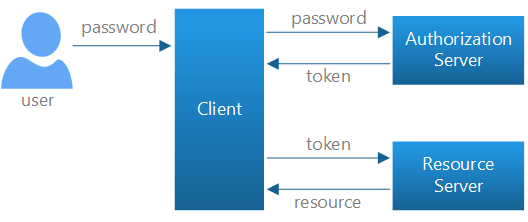
\includegraphics[width=90mm]{./img/authentication.png}
\end{figure}

\section{Ontwikkeling van de cross platforme mobiele applicatie}
\subsection{Gedeelde code}
Om de applicaties zo efficiënt mogelijk te ontwikkelen, wordt er code gedeeld tussen de deelprojecten van de 3 mobiele
platformen. Concreet gaat dit over de code die nodig is voor het ophalen van de gegevens uit de webservice. De code wordt gemeenschappelijk
gesteld voor zowel het Android-, als het iOS- en Windows Phone-project. Daarnaast wordt het domeinmodel gemeenschappelijk
gedefinieërd voor de drie mobiele applicaties. In het project gebeurt dit door in ieder deelproject een referentie toe te voegen
naar het gemeenschappelijke project.

\subsubsection{Code om data op te halen uit de REST-api}
De code die volledig gedeeld wordt omwille van de efficientië, is de code om de data op te halen uit de REST-service.
Hieronder vindt u het voorbeeld dat als basis diende voor de ontwikkeling van de cross platforme mobiele applicatie.
De volledige code met uitgebereide stappen om dit voorbeeld te ontwikkelen is beschikbaar op \citet{buildappwithnativeuiusingxamarininvisualstudio2017}.

Ter voorbereiding van de logica om data uit een REST-api op te halen hebben we een klasse nodig die de entiteit uit het
domein van de toepassing voorziet. In dit geval gaat het om de klasse 'Persoon'  met onder andere de velden 'Voornaam', 'Familienaam', 'Geslacht'.
\newpage
\begin{lstlisting}
namespace MobileApp
{
  public class Persoon
  {
    public string Voornaam {get; set;}
    public string Familienaam {get; set;}
    public string Geslacht {get; set;}
  }
}
\end{lstlisting}
Nu deze domeinklasse gedefinieërd is, kunnen we verdergaan met een klasse aan te maken voor het effectief ophalen van
gegevens uit de REST-service. Hierbij is het belangrijk om op te merken dat deze code asynchroon op de main-thread van de
applicatie wordt uitgevoerd. Voorlopig ziet de klasse er als volgt uit:
\begin{lstlisting}
using System.Threading.Tasks;
using Newtonsoft.Json;
using System.Net.Http;
namespace MobileApp
{
  public class DataService
  {
    public async Task<string> getData(string queryString)
    {
      // Implementatie DataService.getData(string queryString)
    }
  }
}
\end{lstlisting}
Nu we de methode gedefinieërd hebben, kunnen we deze verder implementeren.
Deze implementatie zal bestaan uit 2 delen. In eerste instantie wordt de data opgehaald uit de REST-api. Nadien zal de opgehaalde data
omgevormd worden tot objecten van het type ''Persoon''. Dit type is hierboven reeds gedefinieërd.

De volgende code die we toevoegen aan de klasse ''DataService'' onder ''// Implementatie DataService.getData(string queryString)'', is de code om de data als JSON binnen te halen.
Hiervoor moet er eerst een instantie van de klasse HttpClient (uit de namespace System.Net.Http) aangemaakt worden.
\begin{lstlisting}
  HttpClient client = new HttpClient();
\end{lstlisting}
\newpage
Nu de instantie van HttpClient geïnstanceerd is, kan deze gebruikt worden om data op te halen bij de webservice.
Het ophalen van de data gebeurt aan de hand van onderstaande code:
\begin{lstlisting}
  namespace MobileApp
  {
    // Imports statements

    public class DataService
    {
      public async List<Person> getData(string queryString)
      {
        // een instantie van de klasse HttpClient aanmaken
        HttpClient client = new HttpClient();

        // data ophalen uit de webservice
        HttpResponseMessage response = await client.GetAsync(queryString);

        // data converteren naar persoon-objecten
        List<Person> personen = JsonConvert.DeserializeObject<List<Person>>(response);

        // persoon-objecten teruggeven
        return personen;
      }
    }
  }
\end{lstlisting}



\subsection{Platform specifieke code}
De deelprojecten voor de drie mobiele applicaties bestaan enerzijds uit de definitie van de schermen voor de mobiele applicaties.
Deze definitie gebeurt in xml voor Android, xaml voor Windows Phone en storyboard voor iOS.

Anderzijds is er ook de code die de gebruikersevent van de GUI opvangen. In deze code wordt er vervolgens een request gestuurd naar
de api voor authenticatie en data.
 %% 4
\chapter{Framework responsive website}
\label{ch:frameworkresponsivewebsite}
\section{Architectuur van de responsive website}
De architectuur van de responsive webapplicatie is het ASP.NET MVC 5 framework van ~\cite{aspnetmvcoverview}.
MVC \footnote{Model View Controller} is een combinatie van design patterns waarbij de business-logica, de user interface en de controllers de belangrijkste
onderdelen zijn. De business-logica bestaat uit domein-objecten die op hun beurt de reële situatie waarbinnen de applicatie
gebruikt wordt, weerspiegelt. Het voornaamste doel van het MVC-framework is een scheiding voorzien tussen het grafische
onderdeel van de toepassing (de schermen), de business logica of model en de controllers die instaan voor het delegeren van gegevens
tussen de views en het model. Schematisch ziet het MVC-framework er als volgt uit:
\begin{figure}[ht!]
\centering
\caption{Schematische voorstelling van het MVC-framework \cite{crossplatformmobiledevelopmentinvisualstudio}}
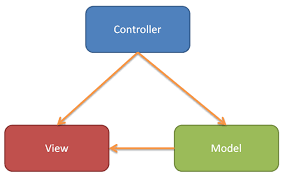
\includegraphics[width=90mm]{./img/mvc.png}
\end{figure}
\section{Voordelen van de gekozen architectuur}
Het ASP.NET MVC 5 framework van ~\cite{aspnetmvcoverview} werd gekozen vanwege volgende voordelen:
\begin{itemize}
  \item Het beheren van complexe applicatie wordt, door de opdeling in Model, View en Controller, eenvoudiger.
  \item Verbeterde ondersteuning voor Test Driven Development \footnote{Test Driven Development is een ontwikkelmethodologie waarbij voorafgaande aan de code eerst de testen geschreven worden. Hierdoor zijn de testen gebaseerd op de oorspronkelijke analyse in plaats van op de geschreven code}
  \item Gecentraliseerde beheer van requests door middel van Front Controller Pattern.
  \item Goede werking voor webapplicaties met grote ontwikkelteams, waarbij de controle over het applicatiegedrag een hoge vereiste is.
\end{itemize}

\section{Nadelen van de gekozen architectuur}
De grootste nadelen van de ASP.NET MVC 5 architectuur zijn volgens ~\cite{hasaspnetcorekilledwebforms} de volgende:
\begin{itemize}
  \item Het moeilijk debuggen van de toepassing in vergelijking met een event-driven variant.
  \item Url's van een ASP.NET MVC 5 applicatie zijn eenvoudiger te begrijpen voor een zoek-robot.
\end{itemize}

\section{Kosten}
Hieronder volgt een overzicht van de voornaamstekosten per fase in de ontwikkeling van de responsive website.
\subsection{Kosten voor de ontwikkeling}
De ontwikkeling van de responsive website is een proces dat niet kostenloos verloopt. Zo moet er een licentie op de ontwikkelomgeving (in dit geval Visual Studio) gekocht worden.
De kosten van deze licentie is afhankelijk van de gekozen. Zo kost een enkele licentie op Visual Studio Professional 2017 499 dollar.

\subsection{Kosten voor testen}
In de testfase zijn er geen kosten verbonden aan de responsive website, aangezien Visual Studio zelf een lokale webserver opzet
voor de hosting van de website. Deze lokale webserver is te bereiken via http://localhost:poortnummer met als poortnummer een
5-cijferig nummer dat vast gekozen is door de ontwikkelomgeving voor de toepassing.
\subsection{Kosten voor publicatie}
Voor de publicatie van de responsive website zijn er volgende optie voor handen:
\begin{itemize}
  \item Men kan kiezen om te hosten op de lokale computer.
  \item Men kan ervoor kiezen om de webapplicatie op een eigen webserver te hosten.
  \item Men kan een externe webserver gebruiken zoals Microsoft Azure.
\end{itemize}
In volgende subsecties worden de kosten zoals electriciteit en koeling van de server buiten beschouwing gelaten omdat deze
mogelijks te grote verschillen opleveren om objectief te kunnen oordelen over de drie publicatiemethoden. Tevens wordt er vanuit
gegaan dat de kosten voor publicatie van de Web api en responsive website gelijk zijn.
%%
\subsubsection{Kosten bij hosting op lokale computer}
De eerste manier van publicatie is het hosten van de webapplicatie op de lokale computer waarop men de responsive website
ontwikkelt. Aan deze manier van publiceren zijn er geen bijkomende kosten verbonden. Het voornaamste nadeel is dat de computer
die de website host, permanent aan dient te staan om de beschikbaarheid te garanderen. Verder is de kost van het installeren
van een webservice minimaal, aangezien die functionaliteit reeds ingebouwd is in de ontwikkelomgeving.
\newpage
\subsubsection{Kosten bij hosting op eigen webserver}
Indien men ervoor kiest om de responsive website op een eigen webserver te hosten, dient men enkel de kosten voor de aankoop en installatie van de webserver in rekening te brengen.
Dit omdat er verder geen kosten zijn voor de hosting van de webserver.

\subsubsection{Kosten bij hosting op externe webserver}
Naast de mogelijkheid om een website zelf te hosten, kan dit ook uitbesteed worden naar een externe service.
Hiervoor worden mogelijks wel kosten voor aangerekend. Bij wijze van voorbeeld vindt u de prijsberekening voor 1 maand Azure hieronder:

  \begin{center}
    \description{Uitgewerkte prijsberekening voor hosting op Azure}
    \newline
  \begin{tabular}{ | l | l | l | l |}
  \hline
  Omschrijving & Region & Prijscategorie & Prijs (€)
  \\ \hline
  SQL Database (Single Database) & West-Europa & Basis & 4,20
  \\ \hline
  API management & West-Europa & Standaard & 41,30
  \\ \hline
  Support & nvt & nvt & 1,33
  \\ \hline
   & & Totaal &  46,83
  \\ \hline
  \end{tabular}
\end{center}
 %% 5
\chapter{Ontwikkeling responsive website}
\label{ch:ontwikkelingresponsivewebsite}
\section{De domeinlaag}
Als eerste stap in de ontwikkeling van de responsive website, is er geopteerd om het business-logica te implementeren.
Dit houdt in dat het opgebouwde domein uit de ASP.NET MVC Web api overgenomen werd in de responsive webapplicatie.

\section{Gebruiken van de bestaande database}
Eens de ontwikkeling van de responsive webapplicatie afgerond is, word deze gekoppeld aan een reeds bestaande databank van de Gentse Politie.
Op deze manier is de reeds aanwezige data direct bruikbaar in de ontwikkelde applicatie.

Om dit tot een goed einde te brengen, wordt er in plaats van "Code-First" de ontwikkelstrategie "Database-First" toegepast in het project.
Zo kan men de webapplicatie en de bestaande database makkelijker op elkaar afstemmen.

\section{Controller voor het tonen van de views}
De controllers hebben een dirigende rol binnen de toepassing, m.a.w. ze verwerken enkel aanvragen vanuit de views en vragen aan onderliggende
klassen gegevens op uit de databank. Die gegevens worden later doorgegeven in de views, die op hun beurt de gegevens in een layout plaatsen om
op een aangename manier weer te geven aan de gebruiker van de toepassing.

\section{Koppeling met Asp Mvc Web api}
Omdat ook in de responsive website-applicatie authenticatie en authorizatie aan de hand van tokens een vereiste is,
dient er een koppeling te zijn tussen de responsive website enerzijds en anderzijds de web api, die tevens door de cross-platform
mobiele applicatie gebruikt wordt.
 %% 6
\chapter{Resultaten cross platforme mobiele applicatie}
\label{ch:resultatencrossplatformapp}
In dit hoofdstuk worden de resultaten van het onderzoek besproken, waarbij er 2 belangrijke
aspecten besproken worden.
Enerzijds wordt de performantie in verband met gegevensgebruik en  snelheid besproken.
Tevens komen ook de tijd die nodig is om de toepassingen te ontwikkelen en de mogelijke
problemen tijdens de ontwikkeling aan bod in de hoofdstuk.
Deze resultaten dienen overigens als basis om later een besluit onder welke
voorwaarden wanneer men best kiest voor de
cross-platforme mobiele applicatie en onder welke voorwaarden men beter kiest voor de responsive website.

\section{Tijd die nodig is om de toepassing te ontwikkelen}
Het eerste gegeven dat in de keuze tussen een cross platforme mobiele
applicatie en responsive webapplicatie van belang is,
is de tijd die nodig is om deze toepassing tot stand te brengen.
Deze tijd wordt samengerekend met de tijd die nodig is om de
REST-api te ontwikkelen. Dit aangezien de REST dient als basis voor de mobiele applicatie.

De eerste stap, in de ontwikkeling van de cross platforme mobiele applicatie, was het opzetten van REST-api.
Deze REST-api heeft een twee-ledige functie, zoals reeds in het Hoofdstuk "Ontwikkeling cross platforme mobiele applicatie" vermeld staat.
Hierbij werd eerst het beschikbaar maken van de data uit een achterliggende databank gerealiseerd. Nadien is de beveiliging aan de hand
van authenticatie-token toegevoegd. De ontwikkeling van deze REST-api heeft ... dagen in beslag genomen. Hieronder vind u in uitgebreid
overzicht van de tijden die de ontwikkeling van de mobiele applicatie.



%% Tabel met tijden invoegen.

\section{Snelheid van de applicatie}

%% Tabel met datagegevens

\section{Gegevensverbruik van de cross platforme mobiele applicatie}
%% Tabel met datagegevens invoegen

\section{Mogelijke problemen bij de ontwikkeling}
Tijdens de ontwikkeling van de cross platforme mobiele applicatie doken er af en toe ook enkele problemen op.
Deze worden ook besproken omdat deze van belang zijn in de keuze tussen de mobiele applicatie en de webapplicatie.

Een eerste zaak die uit het onderzoek naar voor kwam, is dat men bij de ontwikkeling van een iOS-applicatie op windows moet beschikken
over een verbinding tussen een windows-pc en een macOS-toestel. Deze verbinding is noodzakelijk voor enerzijds het kunnen weergeven van
het storyboard of de user interface en anderzijds om de applicatie te kunnen debuggen. Naast het feit dat de structuur van de applicatie
soms moeilijk te begrijpen is in vergelijking met de andere mobiele platformen (Android en Windowsphone), viel ook de verbinding soms weg.
Dit maakt het uiteraard niet eenvoudig om de iOS-applicatie te ontwikkelen.
 %% 7
\chapter{Resultaten responsive website}
\label{ch:resultatenresponsivewebsite}
\section{Tijd die nodig is om de toepassing te ontwikkelen}
Aangezien de tijd die nodig is om de toepassing te ontwikkelen bij de cross platforme mobiele applicatie gemeten wordt,
is dit ook een vereiste voor de responsive webapplicatie. Dit om later een objectieve conclusie te kunnen trekken.
Ook hierbij rekent ook de tijd voor de ontwikkeling van de REST api mee. Deze ontwikkeling nam 7 dagen in beslag.

Na de ontwikkeling van de REST api ging de ontwikkeling van de responsive webapplicatie van start.
Dit duurde 7 dagen, wat de totale ontwikkelingstijd van de responsive website samen met de koppeling tussen de responsive webapplicatie
en de REST api op 15 dagen brengt. De voornaamste redenen dat de ontwikkeling van de responsive webapplicatie sneller verliep in vergelijking met de cross platforme mobiele zijn de volgende:
\begin{itemize}
  \item Betere kennis van en meer ervaring met ASP.NET MVC Webapplicatie.
  \item De uniforme manier van definiëren van de user interface.
\end{itemize}

\section{Snelheid van de applicatie}
Zoals reeds in de methodologie aangegeven, wordt de snelheid van de applicatie gemeten aan de hand van een stopwatch ingebouwd in C\#.
Deze stopwatch wordt gestart wanneer de aanvraag in de juiste controller en wordt gestopt wanneer men de html en css terugstuurt naar de browser.

Om een betere vergelijking te kunnen maken tussen de mobiele applicatie en de responsive webapplicatie, worden beide resultaten vermeld.

\begin{center}
\addcontentsline{lot}{table}{Gemiddelde tijden van de responsive webapplicatie voor inloggen, gegevens ophalen en tonen}
\begin{tabular}{| l | l | l | | l | l }
  \hline
  Statistieken & Android & Windowsphone \\ \hline
  Gemiddelde & 6.552,9562 & 2361,3135 \\ \hline
  Standaardafwijking & 2.657,2925 & 407,9001 \\
  \hline
\end{tabular}
\end{center}

\section{Gegevensverbruik van de responsive website}
In de vergelijking tussen een mobiele applicatie en responsive website, is de hoeveelheid verbruikte data ook een parameter in de beslissing
Het gegevensverbruik van de responsive website wordt gemeten door in de browser de opgehaalde hoeveelheid gegevens te bekijken.
De hoeveelheid data (transferred) en de hoeveelheid gegevens van het DOM \footnote{Document Object Model} wordt hierbij samengeteld.

\begin{center}
\addcontentsline{lot}{table}{Gemiddeld gegevensverbruik van de responsive webapplicatie voor inloggen, gegevens ophalen en tonen}
\begin{tabular}{| l | l | l |}
  \hline
  Statistieken & Android & windowsphone \\ \hline
  Gemiddelde & 596,85 & 885,2 \\ \hline
  Standaarafwijking & 19,2826 & 18,3004 \\ \hline
\end{tabular}
\end{center}
\section{Mogelijke problemen van de responsive website}
De ontwikkeling van de responsive website verliep over het algemeen vlotter dan de ontwikkeling van de cross platforme mobiele applicatie.
Dit is te verklaren door de betere kennis en meer ervaring in het ontwikkelen van responsive website.
Verder werd er eerst zonder de REST api gewerkt, hetgeen de tijd die nodig is om de ontwikkeling te voltooien laat stijgen.
Overigens zijn er geen noemenswaardige problemen tijdens de ontwikkeling van de responsive website opgedoken.
 %% 8
%%=============================================================================
%% Conclusie
%%=============================================================================

\chapter{Conclusie}
\label{ch:conclusie}

%% TODO: Trek een duidelijke conclusie, in de vorm van een antwoord op de
%% onderzoeksvra(a)g(en). Wat was jouw bijdrage aan het onderzoeksdomein en
%% hoe biedt dit meerwaarde aan het vakgebied/doelgroep? Reflecteer kritisch
%% over het resultaat. Had je deze uitkomst verwacht? Zijn er zaken die nog
%% niet duidelijk zijn? Heeft het ondezoek geleid tot nieuwe vragen die
%% uitnodigen tot verder onderzoek?

%%\lipsum[76-80]

%% Snelst resultaat -> website -> beter kennis

%% efficiënst data -> app -> kan nog verder geoptimaliseerd worden mits caching van data

%% snelst gevraagde gegevens -> app -> invloed van caching moet verder ontzocht worden

%% Vermelden dat alle resultaten zonder caching zijn gemeten en dit in de
%% toekomst verder onderzocht kan/moet worden om een preciezere conclusie
%% te kunnen trekken. Hiervoor dient wel de Web api aangepast te worden zodat
%% men alle gegevens na een bepaalde persoon kan opvragen.

%% ook vermelden dat voor het iOS project enkel het inloggen gerealiseerd is.

In dit werk werd een vergelijkende studie en proof-of-concept in functie van een doelbewuste keuze tussen een
cross platforme mobiele applicatie en een responsive website opgezet.

Hierbij werden verschillende aspecten van de ontwikkeling
en de toepassing onderzocht. Hierbij kwamen volgende onderzoeksvragen aan bod:

\begin{itemize}
  \item{Bij welke vorm van applicatie wordt het snelst resultaat behaald?}
  \item{Welke optie is het efficiënst?}
  \begin{itemize}
    \item{Welke optie verbruikt de meeste hoeveelheid gegevens?}
    \item{Welke optie geeft de eindgebruiker het snelst de gevraagde informatie?}
  \end{itemize}
\end{itemize}

Het gevoerde onderzoek leerde ons dat de responsive webapplicatie op de eerste onderzoeksvraag, een beter resultaat haalt dan de mobiele applicatie.

Dit wegens de betere kennis van responsive webapplicatie. Mogelijks verschilt dit van ontwikkelaar tot ontwikkelaar,
afhankelijk van de ervaring met beide technologieën.

Verder moet men ook in overweging nemen dat bij de ontwikkeling van de mobiele applicatie, men voor elk mobiel besturingssysteem een afgeslankte mobiele toepassing dient te ontwikkelen.

Dit doet de ontwikkeltijd oplopen in vergelijking met de responsive website.

Over de efficientie van de mobiele applicatie en de responsive webapplicatie is er wel een duidelijk voordeel voor de mobiele applicatie.
De reden hiervoor is dat het gegevensverbruik lager is bij de responsive website.
Bij de tijden valt echter op dat deze bij Android hoger bij de mobiele applicatie. Dit in tegenstelling tot windowsphone, waar de tijden voor de mobiele applicatie onder die van de responsive website liggen.

Dit is te verklaren omdat er bij de mobiele applicatie enkel de weer te geven data moet gedownload worden. Dit in tegenstelling tot de responsive website, waarbij er naast de weer te geven data, ook nog html
en css gedownload moet worden om de data op een geschikte manier te tonen.

Het resultaat van de mobiele applicatie kan mogelijk nog verder geoptimaliseerd worden vermits in deze casus het effect op het resultaat van cachen of lokaal opslaan van gegevens niet onderzocht is.

Om het lokaal opslaan van data optimaal te laten functioneren, dient de REST api aangepast te worden.

Op de vraag welke optie de eindgebruiker het snelst de gevraagde gegevens, blijkt er geen eenduidige voorkeur uit het onderzoek voort de vloeien.
Dit omdat uit de testresultaten bij Android blijkt dat de respsonive webapplicatie hier beter functioneert. Dit in tegenstelling tot windowsphone, waar de mobiele applicatie betere
resultaten behaald.

Verder dient men ook rekening te houden dat er voor iOS slechts een minimale applicatie ontwikkeld werd.

Om in de toekomst een meer accuraat antwoord te geven op deze onderzoeksvragen, moet het caching van data in de mobiele applicatie voorzien worden.
Dit is momenteel nog niet geïmplementeerd wegens tijdsgebrek.
 %% 9

%%---------- Back matter ------------------------------------------------------

\bibliographystyle{apa}
\bibliography{tin-bachproef}

\listoffigures
\listoftables

\end{document}
